\documentclass[svgnames,dvipsnames,hyperref={bookmarks=false},usepdftitle=false]{beamer}
\usetheme{scalasphere}

\title{What Did We Learn In Scala.Meta?}
\author{Eugene Burmako}
% \institute{
\includegraphics[height=2cm]{epfl.png}}
\institute{\'Ecole Polytechnique F\'ed\'erale de Lausanne \\ \texttt{http://scalameta.org/}}
\date{11 February 2016}
\hypersetup{pdfauthor={Eugene Burmako},pdftitle={What Did We Learn In Scala.Meta?}}

\begin{document}

\titleframe

\begin{frame}[c, fragile]{A big experiment (Berlin 2014)}
\begin{center}

\includegraphics[height=7.5cm]{nx01-therealthing.jpg}
\end{center}
\end{frame}

\begin{frame}[c, fragile]{Initial practical results (San Francisco 2015)}
\begin{center}

\includegraphics[height=5cm]{nx-alpha.jpg}
\end{center}
\end{frame}

\begin{frame}[c, fragile]{Theoretical discussion (Krakow 2016)}
\begin{center}
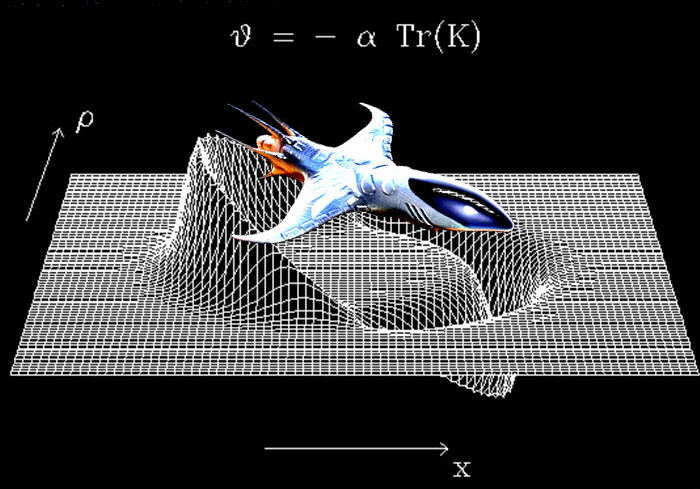
\includegraphics[height=7.5cm]{warp-physics.png}
\end{center}
\end{frame}

\begin{frame}{In this talk}
Q: What did we learn in scala.meta?\\
A: How to design better ASTs.
\end{frame}

\sectionframe{Syntax}

\begin{frame}{Problem (scala.reflect)}
Trees can't precisely represent Scala's syntax
\end{frame}

\begin{frame}[fragile]{Lossy representation (scala.reflect)}
\begin{semiverbatim}
scala> val forLoop = q"for (x <- List(1, 2, 3)) yield x * x"
forLoop: Tree = List(1, 2, 3).\alert<2>{map}(\alert<3>{((x) => x.\$times(x))})

\only<2->{scala> showRaw(forLoop)}
\only<2->{res0: String = Apply(}
\only<2->{  Select(}
\only<2->{    Apply(Ident(TermName("List")), ...),}
\only<2->{    \alert<2>{TermName("map")}),}
\only<2->{  List(}
\only<2->{    \alert<3>{Function(}}
\only<2->{      \alert<3>{List(ValDef(Modifiers(PARAM), TermName("x"), ...)),}}
\only<2->{      \alert<3>{Apply(}}
\only<2->{        \alert<3>{Select(Ident(TermName("x")), TermName("\$times")),}}
\only<2->{        \alert<3>{List(Ident(TermName("x")))))))}}
\end{semiverbatim}
\end{frame}

\begin{frame}[fragile]{Lax representation (scala.reflect)}
\begin{semiverbatim}
scala> val List = \text{\color<2>{red}{tq"scala.List"}}
List: Select = scala.List

scala> val list = \text{\color<2>{blue}{q"}}\text{\color<2>{red}{\$List}}\text{\color<2>{blue}{(1, 2, 3)"}}
list: Tree = scala.List(1, 2, 3)

scala> toolbox.eval(list)
s.t.r.ToolBoxError: \text{\color<2>{red}{type scala.List}} is not a \text{\color<2>{blue}{value}}
  at s.t.r.ToolBoxFactory\$...apply(ToolBoxFactory.scala:178)
  at s.t.r.ToolBoxFactory\$...apply(ToolBoxFactory.scala:170)
  at s.t.r.ToolBoxFactory\$...apply(ToolBoxFactory.scala:148)
  ...
\end{semiverbatim}
\end{frame}

\begin{frame}[fragile]{Funny representation (scala.reflect)}
\begin{semiverbatim}
scala> q"\alert<1>{class C(x: Int)}"
res0: ClassDef =
\alert<1>{class C} extends scala.AnyRef \{
  <paramaccessor> private[this] val x: Int = _;
  def <init>\alert<1>{(x: Int)} = \{
    super.<init>();
    ()
  \}
\}
\end{semiverbatim}
\end{frame}

\begin{frame}{Consequences (scala.reflect)}
scala.reflect has a lossy, lax and funny representation of Scala syntax:
\begin{itemize}
\item It's impossible to have 100\% robust solutions
\item Every metaprogram needs to know about funny encodings
\item Complexity estimate: SyntacticXXX extractors and supporting infrastructure
in the implementation of quasiquotes ($\sim$2kloc)
\end{itemize}
\end{frame}

\begin{frame}{Solution (scala.meta)}
Faithfully model all intricacies of syntax even if it's hard
\end{frame}

\begin{frame}[fragile]
\frametitle<1-4>{Precise representation (scala.meta)}
\frametitle<5>{Safety by construction (scala.meta)}
\begin{semiverbatim}
scala> val forLoop = q"for (x <- List(1, 2, 3)) yield x * x"
forLoop: Term = \alert<2>{for} (\alert<3>{x <- \alert<5>{List}(1, 2, 3)}) \alert<2>{yield} \alert<4>{x * x}

\only<2->{scala> forLoop.show[Structure]}
\only<2->{res0: String = \alert<2>{Term.ForYield}(}
\only<2->{  Seq(\alert<3>{Enumerator.Generator(}}
\only<2->{    \alert<3>{Pat.Var.Term(Term.Name("x")),}}
\only<2->{    \alert<3>{Term.Apply(\alert<5>{Term.Name("List")}, ...))}),}
\only<2->{  \alert<4>{Term.ApplyInfix(}}
\only<2->{    \alert<4>{Term.Name("x"),}}
\only<2->{    \alert<4>{Term.Name("*"),}}
\only<2->{    \alert<4>{Nil, Seq(Term.Name("x")))})}
\end{semiverbatim}
\end{frame}

\begin{frame}{Implementation effort}
\begin{itemize}
\item Several months of iterations on AST definitions
\item Several weeks of adapting the old parser to emit new trees
\item GSoC project on implementing quasiquotes for new trees
\item The functionality is self-contained (no changes to the compiler!)
\end{itemize}
\end{frame}

\begin{frame}[c, fragile]{Demo time: Scala code patterns at codacy.com}
\begin{center}
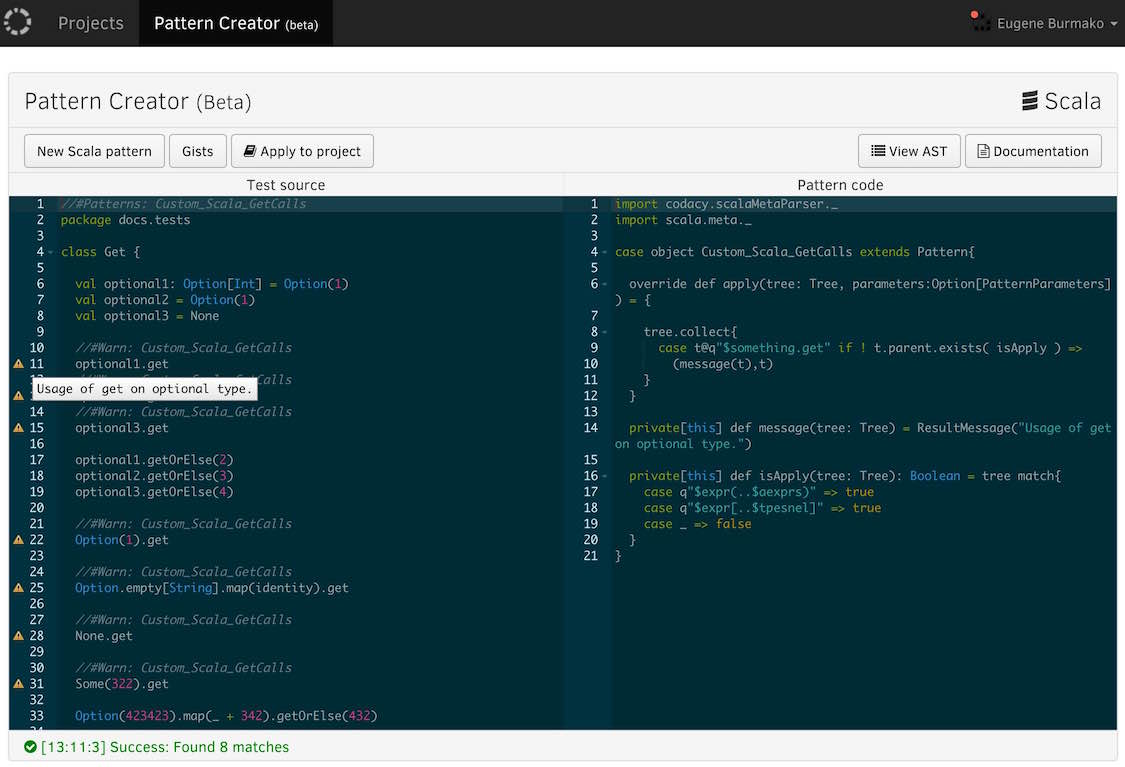
\includegraphics[height=7.5cm]{codacy.jpg}
\end{center}
\end{frame}

\begin{frame}{Challenge \#1: Scala's syntax is hard}
\begin{itemize}
\item Have to model syntactic irregularities
\item Unfortunately there's a bunch of them
\item Constant tension between precise modelling and retaining sanity
\end{itemize}
\end{frame}

\begin{frame}{Challenge \#1: Some examples of irregularities}
\begin{itemize}
\item ``Patterns'' in \texttt{val}/\texttt{var} declarations
\item Pattern variables in type(!) patterns
\item \texttt{new} and super constructor calls
\item ``Names'' in \texttt{private[Foo]} and \texttt{Bar.this} qualifiers
\item ...
\end{itemize}
\end{frame}

\begin{frame}[fragile]{Challenge \#2: Concrete syntax trees are hard}
\begin{semiverbatim}
scala> val q"\$fn(..\$args)" = q"2 + 2"
scala.MatchError: 2 + 2 (of class Term\$ApplyInfix\$Impl)
  ... 33 elided

scala> val q"\$arg \$op (..\$args)" = q"2 + 2"
arg: Term = 2
op: Term.Name = +
args: Seq[Term.Arg] = List(2)

\end{semiverbatim}

\begin{itemize}
\item CSTs are harder to process uniformly than ASTs
\item Need more experience to better understand the trade-offs
\item Maybe there doesn't exist a one-size-fits-all solution
\end{itemize}
\end{frame}

\begin{frame}{Challenge \#3: Need to understand dialects}
\begin{itemize}
\item It's not enough to support just Scala 2.11/2.12
\item Some features are about to be deprecated in future versions
\item Dotty is gaining traction, and it's going to have new features
\end{itemize}
\end{frame}

\sectionframe{Tokens}

\begin{frame}{Problem (scala.reflect)}
Trees can't reflect on underlying lexemes
\end{frame}

\begin{frame}[fragile]{Forgotten trivia (scala.reflect)}
\begin{semiverbatim}
scala> q"\text{\color<1>{red}{/** doc */ }}class C(x: Int)"
res0: ClassDef = class C...
\end{semiverbatim}
\end{frame}

\begin{frame}[fragile]
\frametitle<1>{Can positions be the answer? (scala.reflect)}
\frametitle<2>{There are still problems with trivia (scala.reflect)}
\frametitle<3>{Some lexemes don't have positions (scala.reflect)}
\begin{semiverbatim}
\$ parse \alert<1>{-Xprint-pos} "\text{\color<2>{red}{/** doc */ }}\alert<2>{class C(\text{\color<3>{red}{x}}: Int)}"
[[syntax trees at end of parser]]// Scala source: tmpiIkEYU
\alert<1>{[11:26]}package \alert<1>{[11:11]}<empty> \{
  \alert<1>{\alert<2>{[11:26]}}class C extends \alert<1>{[18:26][26]}scala.AnyRef \{
    \alert<1>{[19:25]}<paramaccessor> private[this] val x: \alert<1>{[22:25]Int} = _;
    \alert<1>{<19:25>}def <init>(\alert<1>{\alert<3>{<19:25>}}x: \alert<1>{[22]}Int) = \alert<1>{<19:25>}\{
      \alert<1>{[NoPosition][NoPosition][NoPosition]}super.<init>();
      \alert<1>{<19:25>}()
    \}
  \}
\}
\end{semiverbatim}
\end{frame}

\begin{frame}{Consequences (scala.reflect)}
scala.reflect ignores trivia and doesn't have fully-featured positions:
\begin{itemize}
\item Tools that want to work on lexical level must reinvent the wheel
\item This hampers the evolution of the tool ecosystem
\end{itemize}
\end{frame}

\begin{frame}{Solution (scala.meta)}
Reify tokens
\end{frame}

\begin{frame}[fragile]{Reified tokens}
\begin{semiverbatim}
scala> "\alert<1,2>{/** doc */} class C(x: Int)".parse[Stat]
res0: scala.meta.Stat = \alert<1,2>{/** doc */} class C\alert<4>{(}\alert<3>{x}\alert<4>{:} Int)

\only<2->{scala> res0.tokens}
\only<2->{res1: scala.meta.tokens.Tokens = Tokens(BOF (0..0),}
\only<2->{\alert<2>{/** doc */ (0..10)},   (10..11), class (11..16),   (16..17),}
\only<2->{C (17..18), \alert<4>{( (18..19)}, \alert<3>{x (19..20)}, \alert<4>{: (20..21)},   (21..22),}
\only<2->{Int (22..25), ) (25..26), EOF (26..26))}
\end{semiverbatim}
\end{frame}

\begin{frame}{Implementation effort}
\begin{itemize}
\item Several days to do the first sketch of tokens
\item Need several more weeks to come up with an optimized representation
\item Several weeks to change the old tokenizer to emit reified tokens
\item Again, the functionality is self-contained
\end{itemize}
\end{frame}

\begin{frame}{Demo time: Scalafmt (created by @olafurpg)}
\begin{center}
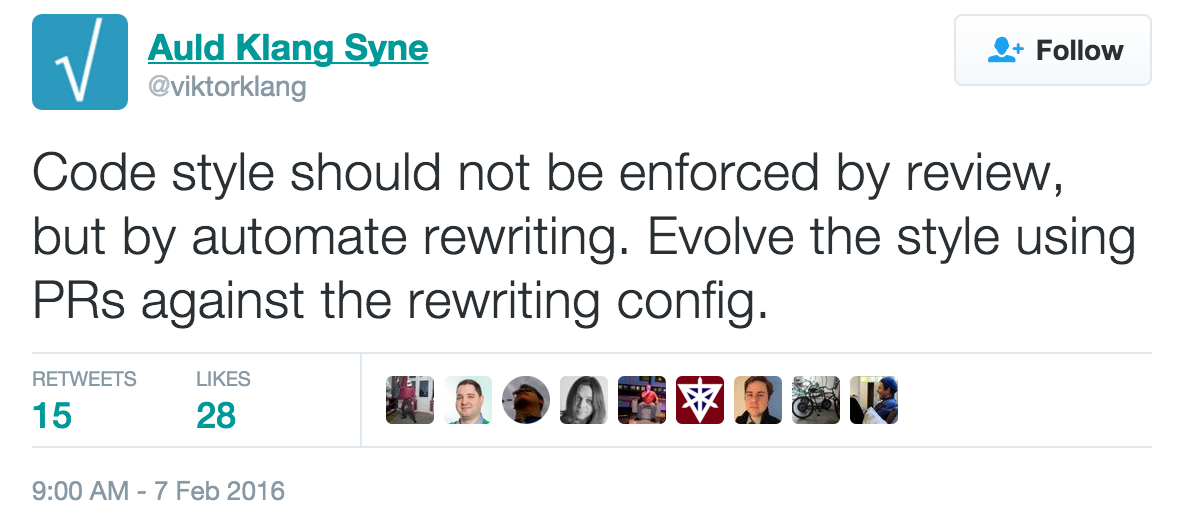
\includegraphics[height=5cm]{klang.png}
\end{center}
\end{frame}

\begin{frame}[fragile]{Demo time: Scalafmt (created by @olafurpg)}
\begin{semiverbatim}
trait Style \{
  def maxColumn: Int = 80
  def indent: Int = 2
  ...
\}

object ScalaFmt \{
  def format(code: String, style: Style): String = ???
\}
\end{semiverbatim}
\end{frame}

\begin{frame}[fragile]{Challenge \#1: Who owns trivia?}
\begin{semiverbatim}
class C \{
  def y = 2

  /** doc */
  def z = 3
\}

\end{semiverbatim}

\begin{itemize}
\item Do tokens for \texttt{y} and \texttt{z} include indentation?
\item What about documentation comments?
\item Roslyn's provides a great practical heuristic
\end{itemize}
\end{frame}

\begin{frame}{Challenge \#2: When to work with tokens?}
\begin{itemize}
\item Working with trees prevents syntax errors
\item However \texttt{clang-format} shows that sometimes that's too high-level
\item How should the low-level API look like?
\item Need more experience to better understand the trade-offs
\end{itemize}
\end{frame}

\sectionframe{Semantics}

\begin{frame}{Problem (scala.reflect)}
Attributed trees have platform-dependent representation
\end{frame}

\begin{frame}[fragile]{Desugaring (scala.reflect)}
\begin{semiverbatim}
scala> val forLoop = q"for (x <- List(1, 2, 3)) yield x * x"
forLoop: Tree = List(1, 2, 3).map(((x) => x.\$times(x)))

scala> toolbox.typecheck(forLoop)
res0: Tree = \alert<1->{immutable.this.}List\alert<1->{.apply[Int]}(1, 2, 3)
.map\alert<1->{[Int, List[Int]]}(((x\alert<1->{: Int}) => x.*(x)))
\alert<1->{(immutable.this.List.canBuildFrom[Int])}

\end{semiverbatim}
\end{frame}

\begin{frame}[fragile]{Desugaring (dotty)}
\begin{semiverbatim}
\$ typecheck 'for (x <- List(1, 2, 3)) yield x * x'
[[syntax trees at end of frontend]]// Scala source: tmpwUlD8P
List\alert<1->{.apply[Int']}(\alert<1->{[}1,2,3\alert<1->{]: Int*}).map\alert<1->{[Int',
  scala.collection.immutable.List[Int']'
]}(\{
  \alert<1->{def \$anonfun(}x\alert<1->{: Int): Int' = }x.*(x)
  \alert<1->{closure(\$anonfun)}
\})\alert<1->{(scala.collection.immutable.List.canBuildFrom[Int'])}
\end{semiverbatim}
\end{frame}

\begin{frame}{Consequences (scala.reflect)}
scala.reflect represents attributed trees in platform-dependent way:
\begin{itemize}
\item Further impairs WYSIWYG metaprogramming
\item Makes it very hard to write portable metaprograms
\item Macros are probably hit the most
\end{itemize}
\end{frame}

\begin{frame}{Solution (scala.meta)}
Platform-independent semantic model
\end{frame}

\begin{frame}[fragile]{Platform-independent semantic model (scala.meta)}
\begin{semiverbatim}
\only<1>{scala> val forLoop = q"for (x <- List(1, 2, 3)) yield x * x"
forLoop: Term = for (x <- List(1, 2, 3)) yield x * x

}scala> forLoop.show[Semantics]
res0: String = \text{\color<4>{teal}{Term.ForYield(}}
  Seq(Enumerator.Generator(
    Pat.Var.Term(\text{\color<2,3>{blue}{Term.Name("x")}}\text{\color<2>{blue}{[1]}}\text{\color<3>{blue}{\{1\}}}<>),
    Term.Apply(\text{\color<2,3,4>{red}{Term.Name("List")}}\text{\color<2>{red}{[2]}}\text{\color<3>{red}{\{2\}}}\text{\color<2>{red}{<1>}}, ...))),
  Term.ApplyInfix(
    \text{\color<2,3>{blue}{Term.Name("x")}}\text{\color<2>{blue}{[1]}}\text{\color<3>{blue}{\{1\}}}<>,
    \text{\color<2>{teal}{Term.Name("*")}}\text{\color<2>{teal}{[3]}}\{4\}<>,
    Nil, Seq(\text{\color<2,3>{blue}{Term.Name("x")}}\text{\color<2>{blue}{[1]}}\{1\}<>))\text{\color<3>{blue}{\{1\}}}<>)\{3\}\text{\color<4>{teal}{<2>}}
\only<1>{...}\only<2>{\text{\color<2>{blue}{[1] \{0\}::local#4efdc590-bcf6-4980-8ad3-06932cb59446}}
\text{\color<2>{red}{[2] \{5\}::scala.collection.immutable.List}}
\text{\color<2>{teal}{[3] \{6\}::scala#Int.*(I)I}}
...}\only<3>{...
\text{\color<3>{blue}{\{1\} Type.Name("Int")[4]}}
\text{\color<3>{red}{\{2\} Type.Singleton(Term.Name("List")[2]\{2\}<1>)}}
...}\only<4>{...
\text{\color<4>{red}{<1> Term.ApplyType(Term.Name("List")[2]\{7\}<3>, ...Int...)}}
\text{\color<4>{teal}{<2> Term.Apply(Term.Apply(...), ...)}}
...}
\end{semiverbatim}
\end{frame}

\begin{frame}{Implementation effort}
\begin{itemize}
\item Several months working on the v1 of the converter
\item Start from scratch
\item Several months working on the v2 of the converter
\item Still can handle only fairly basic programs
\item Maintainability??
\end{itemize}
\end{frame}

\begin{frame}{Challenge \#1: Implementation strategy}
\begin{tabular}{ | l | l | l | l | }
  \hline
  & Difficulty & Reliability & Overhead \\ \hline
  Compiler plugin & Very hard & Brittle & None \\ \hline
  Compiler module & Very hard & Moderate & Moderate \\ \hline
  Integrated into typer & Hard & Robust & High \\
  \hline
\end{tabular}
\end{frame}

\begin{frame}[fragile]{Challenge \#2: When to desugar?}
\begin{semiverbatim}
scala> val forLoop = q"for (x <- List(1, 2, 3)) yield x * x"
forLoop: Tree = List(1, 2, 3).map(((x) => x.\$times(x)))

scala> toolbox.typecheck(forLoop)
res0: Tree = immutable.this.List.apply[Int](1, 2, 3)
.map[Int, List[Int]](((x: Int) => x.*(x)))
(immutable.this.List.canBuildFrom[Int])

\end{semiverbatim}

\begin{itemize}
\item Sometimes need original trees
\item Sometimes need desugared trees
\item On-demand desugaring seems reasonable
\end{itemize}
\end{frame}

\begin{frame}{Challenge \#3: How to be platform-independent?}
\begin{itemize}
\item Even if we desugar on demand, that's still platform-dependent
\item Unless we have a detailed spec of the typechecker
\item (Probably not going to happen)
\end{itemize}
\end{frame}

\sectionframe{What did we learn in scala.meta?}

\begin{frame}{Summary}
\begin{itemize}
\item Almost all scala.reflect problems can be solved by better ASTs
\item<2-> The rest can be reduced to AST problems
\item<3-> And then solved
\end{itemize}
\end{frame}

\begin{frame}{Summary}
It's definitely worth it to have richer parse trees:
\begin{itemize}
\item Concrete syntax trees are essential for writing robust metaprograms
\item Reified tokens enable new kinds of useful tools
\item Implementation complexity is moderate and isolated
\end{itemize}
\end{frame}

\begin{frame}{Summary}
Attributing parse trees is very useful but very hard:
\begin{itemize}
\item Finally provides a way to write macros in WYSIWYG style
\item And makes it possible to develop robust frontend tooling
\item Implementation complexity goes through the roof
\item This is the biggest open question in scala.meta right now
\end{itemize}
\end{frame}

\begin{frame}{Credits}
\begin{tabular}{p{0.4\textwidth}p{0.5\textwidth}}
\begin{itemize}
\itemsep0.5em
\item Uladzimir Abramchuk
\item Eric Beguet
\item Igor Bogomolov
\item Eugene Burmako
\item Mathieu Demarne
\item Martin Duhem
\item \'Olafur P\'all Geirsson
\item Adrien Ghosn
\item Zhivka Gucevska
\item Vojin Jovanovic
\item Guillaume Mass\'e
\end{itemize} &
\begin{itemize}
\itemsep0.5em
\item Guillaume Martres
\item Mikhail Mutcianko
\item Dmitry Naydanov
\item Artem Nikiforov
\item Vladimir Nikolaev
\item Martin Odersky
\item Oleksandr Olgashko
\item Alexander Podkhalyuzin
\item Jatin Puri
\item Dmitry Petrashko
\item Valentin Rutz
\item Denys Shabalin
\end{itemize} \\
\end{tabular}
\end{frame}

\end{document}